
\documentclass[conference]{IEEEtran}

\ifCLASSINFOpdf
 
\else

\fi

\hyphenation{op-tical net-works semi-conduc-tor}

\usepackage{graphicx}
\usepackage{tabularx}
\begin{document}

\title{Internal Ballistics Simulation Based on \\Object Oriented Programming}

\author{\IEEEauthorblockN{Roongtawan Laimek}
\IEEEauthorblockA{Department of Research and Development\\
Defence Technology Institute, Ministry of Defence\\Nonthaburi, Thailand\\
Email: roongtawan.l@dti.or.th}
\and
\IEEEauthorblockN{Wichai Pawgasame}
\IEEEauthorblockA{Department of Research and Development\\
Defence Technology Institute, Ministry of Defence\\Nonthaburi, Thailand\\
Email: wichai.p@dti.or.th}}





% use for special paper notices
%\IEEEspecialpapernotice{(Invited Paper)}




% make the title area
\maketitle


\begin{abstract}
%\boldmath
Internal ballistics simulation involves complex calculation of thrust profile generated by burning solid propellant mass. The design of appropriate solid propellant mass for desired thrust profile requires visualization of propellant mass and overlook how it burns from the start to the end. The use of objected-oriented programming in internal ballistics simulation is introduced in this paper to solve complex calculation of thrust profile and visualise of burning solid propellant. JAVA programming language is chosen to implement a test program for proving internal ballistics simulation. The result shows the reasonable trend of thrust profile according to the real behavior of thrust generated by solid propellant. This paper give intuitive idea of applying object-oriented programming in internal ballistics simulation.
\end{abstract}

\IEEEpeerreviewmaketitle



\section{Introduction}

Due to many different types of rockets require different thrust profile for difference purpose, Designing of rocket propellant is necessary in order to archive suitable rocket propellant. This is a complex task and hard to be done by hand. Therefore software is necessary as a tool to design a complex rocket propellant. In many country researches have been conducted to develop suitable software. However this kind of software affects the national security and cannot be released outside their country. In Thailand some researches on rocket propellant cannot support complex design of rocket propellant. Thereby research on this topic would be valuable in term of economic and security of country.

The paper in [1] presents the use of computer program to design rocket propellant. However the program is limited to design rocket propellant of only 2 layers. In addition it lacks of capability to visualize the rocket propellant design. The geometry of rocket propellant has to be designed in external CAD programs. Object Oriented Programming (OOP) is a programming language model organized around objects rather than actions and data rather than logic. [2] Hence we can model each layer of rocket propellant as object in OOP which make complex calculation of thrust profile easier.

In the next section, we discuss background information and previous studies related to Internal Ballistics simulation. Section II explains the OOP design and implementation of the Internal Ballistics. Section IV presents result of the pilot program to prove our propose concept, and discussed in section V. Section VI concludes and presents future improvements.

\begin{figure*}[t]
\centering
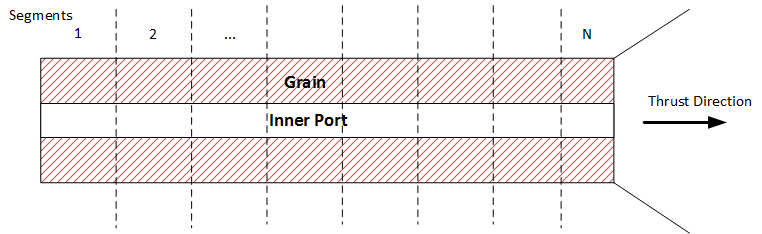
\includegraphics[width=0.8\textwidth]{propellant_cut}
\caption{Burning surface layer at 2 mm distance of solid propellant grain}
\label{fig:2_1}
\end{figure*}

\section{Background and Related Works}
Inside Rocket Motor stored propellant mass, which drive the rocket forward. The combustion process proceeds throughout the length of the chamber and generate hot gases flow through the nozzle at high speed. Hence, thrust force is produced at the nozzle end.

 Solid-propellant rocket is the simplest of all rocket design. Unlike liquid-propellant engines, solid-propellant motors can’t be shut down. Once ignited, they burn until all the propellant is exhausted [3],  we can’t control the thrust force so designing of rocket propellant is necessary in order to archive suitable thrust profiles. Mostly propellants are designed with difference shapes of inner port. Calculating Cross section area is important to design rocket propellant efficiently.
 
There are two types of solid propellant, Double-Base propellant consist mainly of fibrous nitro-cellulose and a gelatiniser, or plasticiser, such as nitro-glycerine or a similar compound (ethylene glycol dinitrate), each containing oxygen and fuel in the same compound.[4] Composite propellant are solid particles of oxidizer and fuel suspended in a binder. The binder is liquid when cast into the rocket chamber and sets up or cures to form a rubbery compound.[5] The simulation program proposed in this paper only consider Composite propellant.

The principle method of the propose program is to calculate the mass flow rate of the generated gas at the nozzle using iteration method along with the geometric data of inner port shape of the solid propellant.

The basic principle of mass flow rate calculation can be found in [6] The calculation assume that a rocket is in a steady state that is
\begin{center}
\begin{equation}
\dot{m}_{NOZZ} = \dot{m}_{p}
\end{equation}
\end{center}
$\dot{m}_{NOZZ}$ = Mass flow rate at the nozzle\\
$\dot{m}_{p}$ = Mass flow rate generated from propellant combustion\\		

The relationship between Mass flow rate at the nozzle and Pressure at the nozzle.
\begin{center}
\begin{equation}
\dot{m}_{NOZZ} = P{A}_tC^{*}
\end{equation}
\end{center}
$P$ = Pressure at the nozzle\\
${A}_t$ = Cross section area of the nozzle\\		
$C^{*}$ = Characteristic Velocity of propellant\\

Mass Flow Rate generated from propellant combustion is calculated from this equation. 
\begin{center}
\begin{equation}
\dot{m}_{p} = \int\rho{r}_bdA
\end{equation}
\end{center}
$\rho$ = Density of propellant\\
${r}_b$ = Burning rate of solid propellant\\		
$A$ = Burning area of solid propellant\\

For the composite propellant burning rate (${r}_b$) is a function of pressure  
\begin{center}
\begin{equation}
{r}_b = aP^{n}
\end{equation}
\end{center}
$a$ = Pre-exponential Factor\\ 
$n$ = Pressure Exponent \\		

In addition to burning rate given by equation (4) we account for erosive burning component which make the burning rate become 
\begin{center}
\begin{equation}
{r}_b = aP^{n} + \alpha G^{0.8}D^{-0.2}exp(-c\beta{r}_b\rho/G)
\end{equation}
\end{center}
$G$ = Mass Flow Rate per cross section area of $Port = \dot{m}_{p}/{A}_p$\\
${A}_p$ = Cross section area of port\\		
$D$ = Characteristic Dimension of $Port = 4{A}_p/S$ \\
where $S$ = Port periphery, \\
$\alpha$ and $\beta$ are Empirical constant usually $\beta = 53$



\section{Design and Implementation}

\subsection{Thrust Calculation}
We divide propellant mass into several segments as illustrated in figure . Thrust Profile is calculated from mass flow rate of generated gas at the nozzle. 

Mass flow rate at the nozzle is calculated from the mass flow rate from previous segments.

Mass flow rate in each segment is calculated as 
\begin{center}
\begin{equation}
\dot{m}_{i} = \dot{m}_{i-1}+{m}_{gen\_i}
\end{equation}
\begin{equation}
{m}_{gen\_i} = \rho\cdot{r}_b(P,\dot{m}_{i})\cdot{A}_i
\end{equation}
\end{center}
${m}_{gen\_i}$ = Mass flow rate of generated gas in segment i\\
${r}_b$ = Burning rate with erosive burning as a function of pressure and total mass flow rate flowing out from segment i\\		
${A}_i$ = Cross section area of throat in segment i\\

In calculation cross section area and periphery in the segment is a function of burning distance from the previous surface. 

To calculate guess pressure and start calculate from the first segment. Assume that mass flow rate into the first segment equal mass flow rate of igniter. 	
\begin{center}
\begin{equation}\dot{m}_{0} = \dot{m}_{igniter}(t)
\end{equation}
\end{center}
where $t \leq$ burning time of igniter\\
$\dot{m}_{igniter} = \dot{m}_{igniter}/(t)$\\
where t $>$ burning time of igniter ; $\dot{m}_{igniter}=0$\\

Mass flow rate at segment i is calculated by 
\begin{center}
\begin{equation}
\dot{m}_{i} = \dot{m}_{i-1}+\rho{r}_{b1}(P,(\dot{m}_{i}+\dot{m}_{i-1})/2)A(\xi)
\end{equation}
\end{center}

Mass flow rate at segment N is equal to Mass flow rate at the end of nozzle.
\begin{center}
\begin{equation}
\dot{m}_{N} = \dot{m}_{p}
\end{equation}
\end{center}

Verify if $P$ from $\dot{m}_{N} = \dot{m}_{p}= \dot{m}_{Nozz}= P{A}_tC^{*}$ is equal to guessed $P$, use $P$ to iterate until guessed $P$ is closed to Convergence Limit.

Use $P$ to calculate thrust at the nozzle[6] 
	
\begin{center}
\begin{equation}
F={C}_FP{A}_t
\end{equation}
\end{center}
where ${C}_F$ = Thrust coefficient


\begin{figure}[t]
\centering
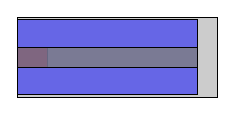
\includegraphics[width=0.3\textwidth]{horizontal_cut}
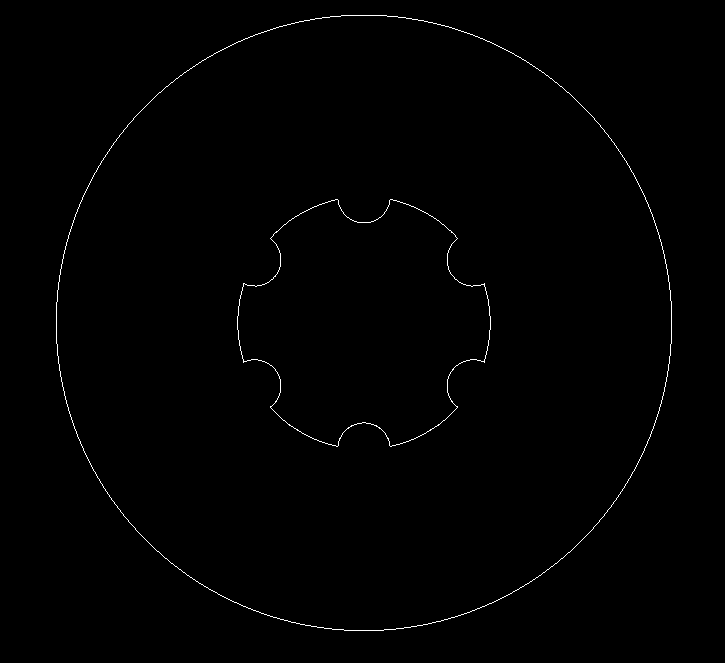
\includegraphics[width=0.4\textwidth]{cross_section}
\caption{Cross-section and horizontal cuts of solid propellant's grain}
\label{fig:1}
\end{figure}

\begin{figure}[t]
\centering

\includegraphics[width=0.4\textwidth]{burnlayer}
\caption{Burning surface layer at 2 mm distance of solid propellant grain}
\label{fig:2}
\end{figure}

\subsection{The role of Object-Oriented Program Architecture}

\subsection{Visualization of Solid Propellant Design}
The key point of designing solid propellant’s grain is a visualization of grain. Figure {\ref{fig:1}} illustrates cross-section cut and horizontal cut of cylindrical grain. The visualization of solid propellant grain illustrates how grain's surface is burnt and generate gas. Computer aided design (CAD) softwares are usually used for designing solid propellant grain. The inner port of the grain is the surface that will burn in the direction perpendicular to previous surface. Figure {\ref{fig:2}} illustrates burning surface at burnt distance of 2 mm. The offset algorithm is useful to generate such layers of burning as illustrated in Figure {\ref{fig:2}} {\cite{offset}}. In addition, most of CAD softwares have the capability of measuring inner port's periphery and area, which are used in thrust profile calculation.   




\begin{figure*}[t]
\centering
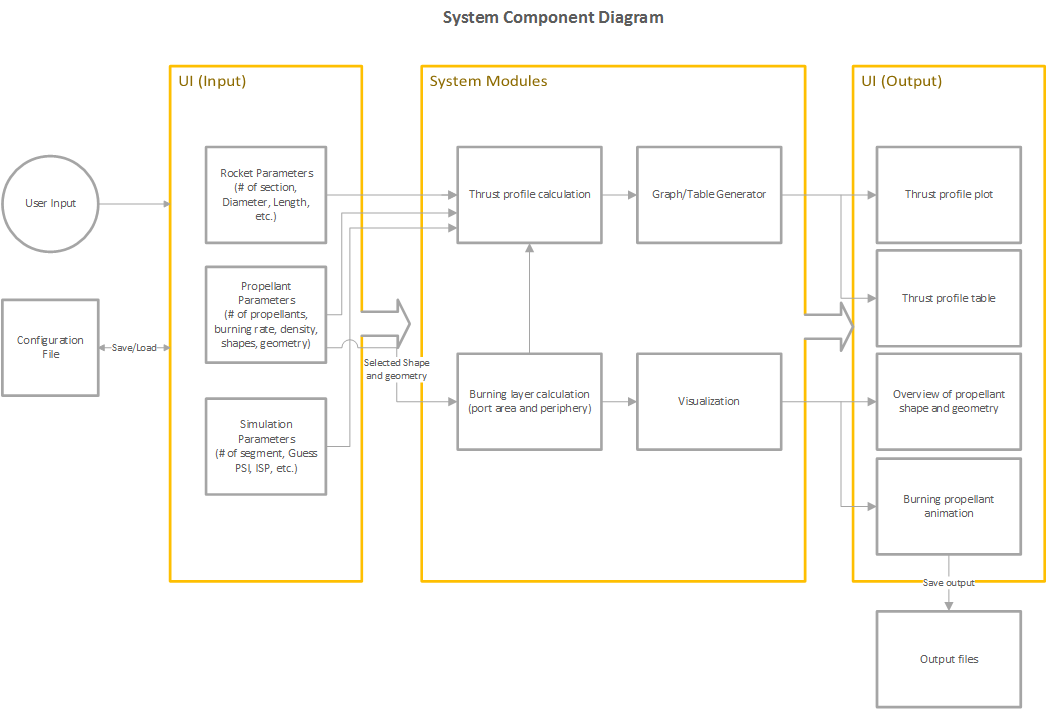
\includegraphics[width=0.9\textwidth]{SystemComponents}
\caption{System Components of the test program}
\label{fig:3}
\end{figure*}
\begin{figure*}[t]
\centering
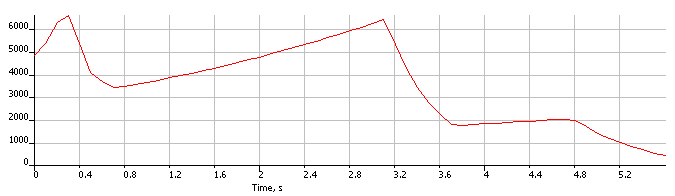
\includegraphics[width=0.9\textwidth]{thrust}
\caption{Thrust profile of simulated propellant grains from the test program}
\label{fig:5}
\end{figure*}

 
\subsection{Program Architecture}
To illustrate the use of OOP in Internal Ballistics simulation, a test program is written in JAVA to calculate thrust profiles of the . Figure {\ref{fig:3}} illustrates the high-level system architecture of the software. More than one solid propellants can be contained in a motor case. Each section can be modeled as an object with different propellant properties and geometries. Each section is then subdivided into small segments during calculation process. The program requires user to specify rocket, propellant, and simulation parameters. The process of calculation is already given in Section III. A CAD software is used to design inner port of the propellant grain, and capture inner port's periphery and area at each burning distance. Inner port's periphery and area data is then imported into the test program for calculation of thrust profile. The output of the test program is calculated thrust and pressure as functions of time. 

\section{Result and Disscussion}
The program was simulated with parameters specified in Table \ref{tab:1}. The simulation assumes two propellant masses placed inside the motor case. Each has the same length and propellant's properties. Each section of propellant mass contains single layer of propellant. 
\begin{table}[h]
  \renewcommand{\arraystretch}{2}
  \renewcommand{\tabcolsep}{1.5mm}
  \centering
  \begin{tabularx}{0.5\textwidth}{|X|X|}
    \hline
    \multicolumn{1}{|c|}{\textbf{Parameters}} &  
    \multicolumn{1}{c|}{\textbf{Values}} \\ \hline
    \textbf{Rocket Length (\(m\))} &  \multicolumn{1}{c|}{2.2} \\ \hline 
    \textbf{Rocket Throat Diameter (\(mm\))} &  \multicolumn{1}{c|}{81} \\ \hline 
    \textbf{Number of propellant mass} &  \multicolumn{1}{c|}{2} \\ \hline 
    \textbf{Number of Segments} &  \multicolumn{1}{c|}{100} \\ \hline 
    \textbf{Shape of inner port} &  \multicolumn{1}{c|}{Wheel} \\ \hline 
    \textbf{Number of propellant layer} &  \multicolumn{1}{c|}{1} \\ \hline 
    \textbf{Burning Rate (\(kg/s\))} &  \multicolumn{1}{c|}{0.011} \\ \hline 
    \textbf{Pressure Exponent} &  \multicolumn{1}{c|}{0.48} \\ \hline 
    \textbf{Density (\(kg/m^{3} \))} &  \multicolumn{1}{c|}{0.001795} \\ \hline 
    \textbf{Erosive Burning Constant} &  \multicolumn{1}{c|}{ \(60 \times 10^{-7}\) } \\ \hline
    \textbf{Gas temperature (\(K\))} &  \multicolumn{1}{c|}{ 3500 } \\ \hline 
    \textbf{Individual Gas Constant} &  \multicolumn{1}{c|}{ 308 } \\ \hline 
    \textbf{Heat Capacity Ratio} &  \multicolumn{1}{c|}{ 1.2 } \\ \hline 
    \textbf{Specific Impulse} &  \multicolumn{1}{c|}{ 265 } \\ \hline 
    \textbf{Guess Pressure (\(PSI\))} &  \multicolumn{1}{c|}{ 1200 } \\ \hline 
  \end{tabularx}
  \space
  \caption{Summary of simulation parameters}
  \label{tab:1}
\end{table}
During calculation, propellent masses is divided into small segments and mass flow rates of each segment is calculated as mentioned in Section II. The simulation uses 100 segments. More segments would give more precise calculation, but requires longer calculation time. Mass flow rate at the nozzle is the consecutive sum of mass flow rate from each segment. The result of thrust profile is shown in Figure {\ref{fig:5}}. 



The peak at the beginning of the plot is the result of mass flow rates of igniter and propellant masses. As the igniter has gone out, thrust starts to drop and only propellant masses are burnt. Thrust starts to go up again as more propellant masses are burnt, and it will drop until pressure is below 50 PSI when all propellant masses are burnt out. 



\section{Conclusion}

Simulation of internal ballistics requires complex calculation of thrust profile. The calculation requires many steps of iteration. The use of object-oriented programming helps easy implementation of such complex internal ballistics simulations. The visualization of propellant masses helps designing of solid propellant masses. The designing of propellant grain are usually done in CAD software. CAD software can be used to extract periphery and area of grain's inner port, which will be in calculation of thrust profile. The test program is implemented to verify the use of object-oriented program to simulate internal ballistics of solid propellant. The test program implement theories and algorithm of thrust profile calculation that was previously conducted by other researches. The result shows that object-oriented program can implement complex calculation of internal ballistics. However, the purpose of this reasearch is to introduce the use of object-oriented programming in internal ballistics simulation. Many further studies should be conducted to obtain effective simulation algorithms.            


\begin{thebibliography}{100}

\bibitem{AA}

A.A.Puntambeker, “Advanced Data Structures and Algorithms,” Pune, India: Technical Publications Pune, 2008, pp. 2.

\bibitem{Solid}
“Solid-Propellant Rocket motor”,\emph{ Internet:  $www.daviddarling.info/encyclopedia/S/solid-propellant_rocket_motor.html$}
\bibitem{AB}
Andre Bedard. “Double Base Solid Propellants”, Internet: www.astronautix.com/articles/doulants.htm 
\bibitem{Fre}
“Frequently Asked Questions On Making Your Own Rocket Motors”, Internet: www.space-rockets.com/faq.html, Feb. 23, 2013
\bibitem{GP}
George P. Sutton, “Rocket Propulsion Elements,” New York: John Wiley \& Sons, 1992
\bibitem{offset}
Xu-Zheng Liu, Jun-Hai Yong, Guo-Qin Zheng, Jia-Guang Sun, {\em An offset algorithm for polyline curves }, Computers in Industry, Vol. 58, Issue 3, April 2007, pp. 240-254
\end{thebibliography}


\end{document}


